\documentclass[10pt]{article}

\usepackage{ulem}
\usepackage{multicol}
\usepackage{hyperref}
\hypersetup{
    colorlinks=true,
    linkcolor=blue,
    filecolor=cyan,      
    urlcolor=magenta,
}
\usepackage{color}
\usepackage{graphicx}
\usepackage[edges]{forest}
\usepackage{enumerate}
\usepackage{enumitem}
\usepackage{amsmath, amssymb, mathrsfs, amsthm, mdframed}
\usepackage{algpseudocode}
\usepackage{listings}
\surroundwithmdframed[
  hidealllines=true,
  innerleftmargin=25pt,
  innertopmargin=0pt,
  innerbottommargin=0pt]{lstlisting}
\usepackage{graphicx}
\usepackage{tikz}
\usetikzlibrary{arrows.meta}

\usepackage{xcolor}

\lstdefinestyle{customc}{
  belowcaptionskip=1\baselineskip,
  breaklines=true,
  frame=L,
  xleftmargin=\parindent,
  language=Python,
  showstringspaces=false,
  basicstyle=\footnotesize\ttfamily,
  keywordstyle=\bfseries\color{green!40!black},
  commentstyle=\itshape\color{purple!40!black},
  identifierstyle=\color{blue},
  stringstyle=\color{orange},
}

\lstdefinestyle{customasm}{
  belowcaptionskip=1\baselineskip,
  frame=L,
  xleftmargin=\parindent,
  language=[x86masm]Assembler,
  basicstyle=\footnotesize\ttfamily,
  commentstyle=\itshape\color{purple!40!black},
}

\lstset{escapechar=@,style=customc}
 
\usepackage[margin=2cm]{geometry}
\usepackage{fancyhdr, lastpage, pgfplots}
\usepackage{mathtools}
\DeclarePairedDelimiter\ceil{\lceil}{\rceil}
\DeclarePairedDelimiter\floor{\lfloor}{\rfloor}

\pagestyle{fancy}
\renewcommand\qedsymbol{$\blacksquare$}

\fancyhf{}
\lhead{CSC373H1, Fall 2019}
\rhead{Assignment 3}
\rfoot{Page \thepage/\pageref{LastPage}}

\setlength\parindent{0pt}
\begin{document}

\begin{center}
\Large \textbf{CSC373H1: Assignment 3}

\vspace{1mm}
\large {\href{mailto:junmingpeter.zhang@mail.utoronto.ca?Subject=CSC373H1: Assignment 3}{\textcolor{blue}{Junming Zhang: 1003988982}}\\
        \href{mailto:yuchen.tong@mail.utoronto.ca?Subject=CSC373H1: Assignment 3}{\textcolor{blue}{Yuchen Tong: 1003534669}}\\
        \href{mailto:yuchen.fan@mail.utoronto.ca?Subject=CSC373H1: Assignment 3}{\textcolor{blue}{Yuchen Fan: 1003800265}}}\\

\vspace{1mm}
\large {Due: November 17th, 2019 before 11:59 p.m.}
\end{center}
\section*{Instructions}
\begin{enumerate}
    \item Be sure to include your name and student number with your assignment. Typed assignments are preferred (e.g., PDFs created using LaTeX or Word), especially if your handwriting is possibly illegible or if you do not have access to a good quality scanner. Please submit a single PDF on MarkUS at \url{https://markus.teach.cs.toronto.edu/csc373-2019-09}
    \item You will receive $20\%$ of the points for any (sub)problem for which you write “I do not know how to approach this problem.” (you will receive $10\%$ if you leave the question blank and do not write this or a similar statement). Not applicable to BONUS questions.
    \item You may receive partial credit for the work that is clearly on the right track. But if your answer is largely irrelevant, you will receive 0 points.
    \item This assignment has 4 questions  (worth 20, 10, 20, 20 marks).
\end{enumerate}

\section*{Q1 [20 Points] LP and IP}
Consider the following primal LP and IP in standard form:
\begin{align*}
    &\text{Maximize} \; &x_2\\
    &\text{Subject to} \; &-3x_1 + 5x_2 \leq 8\\
                        & &7x_1 + 3x_2 \leq 12\\
                        & &x_1, \; x_2 \geq 0
\end{align*}
For the IP, add the constraints that $x_1$ and $x_2$ are integers.\\
\\
Plot the feasible region of this program. \textit{Note: You do not need to submit this with the assignment, but it will be helpful to plot the feasible region}. You can use any online graphing programs such as
desmos, fooplot, etc.
\begin{itemize}
    \item [\textbf{(a)}] {[5 Points]} What are the vertices of the feasible region of the primal LP? (No explanation is needed.)
    \begin{mdframed}
        % 1 a)
        \textit{Solution.}\\
        $(\frac{9}{11}, \frac{23}{11}), x_1=\frac{9}{11}, x_2 = \frac{23}{11}\\
        (\frac{12}{7}, 0), x_1=\frac{7}{12}, x_2 = 0\\
        (0, \frac{8}{5}), x_1=0, x_2 = \frac{8}{5}$
    \end{mdframed}
    \item [\textbf{(b)}] {[5 Points]} What are the optimal solutions of the primal LP and IP? What are the corresponding optimal objective values? (No explanation is needed.)
    \begin{mdframed}
        % 1 b)
        \textit{Solution.}\\
        \textbf{LP:} $\frac{23}{11}$, $x_1 = \frac{9}{11}$, $x_2 = \frac{23}{11}$\\
        \textbf{IP:} $1$, $x_1 = 0$, $x_2 = 1$ or $x_1 = 1$, $x_2 = 1$
    \end{mdframed}
    \item [\textbf{(c)}] {[5 Points]} Provide the dual LP of the primal LP above. Clearly indicate which dual variable in your formulation corresponds to which primal constraint.
    \begin{mdframed}
        % 1 c)
        \textit{Solution.}
        \begin{align*}
            \text{multiplier}& \; &\text{Inequality}\\
            y_1& \; &-3x_1 + 5x_2 \leq 8\\
            y_2& \; &7x_1 + 3x_2 \leq 12\\
        \end{align*}
        We have:\\
        $$y_1(-3x_1+5x_2) + y_2(7x_1+3x_2) \leq 8y_1+12y_2$$
        $$(-3y_1+7y_2)x_1 + (5y_1+3y_2)x_2 \leq 8y_1+12y_2$$
        we get:\\
        $y_1 \text{ and } y_2 \geq 0$\\
        $-3y_1+7y_2 \geq 0$, $5y_1+3y_2 \geq 1$\\
        \textbf{Dual LP:}
        \begin{align*}
            &\text{Minimize} \; &8y_1+12y_2\\
            &\text{Subject to} \; &-3y_1+7y_2 \geq 0\\
                        & &5y_1+3y_2 \geq 1\\
                        & &y_1, \; y_2 \geq 0
        \end{align*}
        \textbf{Primal LP:}
        \begin{align*}
            &\text{Maximize} \; &x_2\\
            &\text{Subject to} \; &-3x_1 + 5x_2 \leq 8\\
                        & &7x_1 + 3x_2 \leq 12\\
                        & &x_1, \; x_2 \geq 0
        \end{align*}
    \end{mdframed}
    \item [\textbf{(d)}] {[5 Points]} What are the optimal solutions of the dual LP and its IP version? What are the corresponding optimal objective values? Does strong duality hold for this particular pair of primal and dual IP?
    \begin{mdframed}
        % 1 d)
        \textit{Solution.}\\
        \textbf{Dual LP:} $\frac{56}{44} + \frac{36}{44} = \frac{23}{11}$, $y_1 = \frac{7}{44}$, $y_2 = \frac{3}{44}$\\
        \textbf{Dual IP:} $20$, $y_1 = 1$, $y_2 = 1$\\
        \textbf{It does not hold strong duality for primal and dual IP.\\ Primal IP opt is 1 and dual IP opt is 20. The duality gap is not zero.}
    \end{mdframed}
\end{itemize}

\section*{Q2 [10 Points] Team Building}
You are putting together a team of $m$ players. The $m$ positions in your team are ranked (so there is a position $k$ for every $k \in \{1, 2, ..., m\}$. You can select your players from a pool of n people, denoted $N = \{1, ..., n\}$. Assume $n > m$.\\
\\
Each person $i \in N$ has a celebrity rating $c_i$ and suitability $s_{ik} \in [0, 1]$ that measures how well person $i$ can play in position $k$ on the team, where $k \in \{1, 2, ... , m\}$. You are also given a relation
$I \subseteq N \times N$, where $(i, j) \in I$ indicates that person $i$ and person $j$ are \textit{incompatible}, and should never be put on the team together. You can assume that this relation is symmetric, so $(i, j) \in I$ if and only if $(j, i) \in I$.\\
\\
Your goal is to pick a team that maximizes the total celebrity rating of all selected players, subject to making sure that the total suitability of players for their assigned positions is at least 1 and no pair of players on the team is incompatible.\\
\\
Give an linear or integer programming formulation for choosing the desired optimal team. Please include a high-level verbal description of your program and justify the correctness of your solution.
\begin{mdframed}
    % 2
    \textit{Solution.}\\
    \textbf{Algorithm:}\\
    \\Let $X_i, i \in N$ be the binary array indicates whether player i will be chosen or not.
    \\- if $X_i = 0$, player i will not be chosen.
    \\- if $X_i = 1$, player i will be chosen.
    \\
    \\Let $Y_{ki}, i \in N, k \in M$ be the binary 2D array indicates whether assign position k to player i.
    \\- if $Y_{ki} = 0$, position k will not be assigned to player i.
    \\- if $Y_{ki} = 1$, position k will be assigned to player i.
    \\
    \\Let $I_c[i,j]$ be the binary 2D array indicates whether player i and j are incompatible.
    \\- $I_c[i,j] = 0$, if i = 0 or j = 0. player i or j are not selected for positions.
    \\- $I_c[i,j] = 1$, if player i and j are incompatible, $(i,j) \in I$ 
    \\- $I_c[i,j] = 0$, if player i and j are compatible.
    \\
    \\Maximize: $\sum_{i}^N c_i X_i$
    \\Subject to:
    \\ $\sum_k^M\sum_i^N s_{ik}Y_{ki} \geq 1$
    \\ $\sum_k^m\sum_i^N\sum_j^N I_c[iY_{ki}, jY_{kj}] \leq 0$
    \\
    \\ The first constraints adds up every selected player's suitability, since for all players in N, if player is not selected for job k which means that $Y_{ki} = 0$, then the suitability summation will not change. Hence it only adds up all the selected player's suitability. By the constraints given in the question, the summation of the player's suitability should be greater or equal to 1, which guarantees that the suitability will always greater than or equal to 1 during run time.
    \\
    \\ The second constraints go though current selected team and adds up the compatibility to test whether there is any incompatible pairs. Since if there is a incompatible pair in the team, then the sum will be greater than 1 based on the implementation of the $I_c[i,j]$. According to the constraints given in the question, this second constraints guarantees that there will be no incompatible pairs occurs during run time.\\
    \\
    \\(a) By Modifying the original LP formulation we get a new $LP_2$:
    \\Minimize: $z_1 + z_2$
    \\Subject to:
    \\$\sum_k^M\sum_i^N s_{ik}Y_{ki} - s_1 + z_1= 1$
    \\$\sum_k^m\sum_i^N\sum_j^N I_c[iY_{ki}, jY_{kj}] + s_2 + z_2= 0$
    \\$s \geq 0, z \geq 0$
    \\(b) Solve $LP_2$ using simplex with the initial basic feasible solution Y is all zero, $s_1 = 0, s_2 = 0, z_1 = 1, z_2 = 0$.
    \\- If the optimal solution of $LP_2$ is 0, extract a feasible solution \hat{x} from it. Again using simplex to solve the original LP with initial feasible solution \hat{x} to get the optimal team, return X and Y.
    \\- Otherwise, the LP has no feasible solution, return False.
    \\
    \\
    \\
    \textbf{Proof of correctness:}
    \\
    \\
    \textbf{Proof that the LP is bounded:}
    \\Since $c_i \leq max\{c_i\},i \in N$, $\sum_{i}^N c_i X_i \leq n*max\{c_i\}$
    \\Therefore $\sum_{i}^N c_i X_i$ is bounded above.
    \\
    \\
    \textbf{Proof that the algorithm will produce a feasible solution of LP if it has one:}
    \\By transforming LP to $LP_2$ as above, solving the $LP_2$ is equivalent to testing whether LP has no solution since when $z_1 = 0$ and $z_2 = 0$, the constraints of $LP_2$ is the same as the LP.
    \\(1) When the optimal solution for $LP_2$ is $z_1 + z_2 = 0$:
    \\- Extract $\hat{x}$ from it
    \\- And there is a feasible solution for LP: $\hat{x}$
    \\(2) When the optimal solution for $LP_2$ is greater than 0:
    \\- There is no solution for LP, return false is expected.
    \\
    \\\textbf{Proof that the algorithm produce a optimal solution:}
    \\Since the LP is bounded and it has a feasible solution as previous proof states.
    \\By using simplex algorithm as described in my previous algorithm. 
    \\Providing a feasible solution for the LP and this LP is bounded yields that a optimal solution is guarantee to be found.
    
    
    \end{mdframed}

\section*{Q3 [20 Points] \textit{P} , \textit{NP} , and \textit{coNP}}
For each decision problem below, state whether it belongs to $P$, $NP$, or $coNP$. Make the strongest claim that you can. E.g. if you can show that a problem is in $P$, then you should claim so, as this implies membership in $NP$ and $coNP$. Similarly, e.g., if you think it is not in $P$ but is in both $NP$ and $coNP$, then you should claim so, instead of claiming membership in just one of them. Note that if you claim a problem is in $NP$ or $coNP$, you \textit{do not} have to show $NP-$ or $coNP-$completeness.\\
\\
In all the problems below, you may assume that a cycle in a graph means a \textit{simple} cycle with no repeated vertices. Assume all graphs are undirected. $\mathbb{Z}^+$ is the set of \textit{positive} integers.\\
\\
Justify your answers. If you claim a problem is in $P$, give a polynomial\-time algorithm and argue its correctness and running time. If you claim a problem is in $NP$ and/or $coNP$, then prove this membership.

\begin{itemize}
    \item [\textbf{(a)}] {[5 Points]} \textbf{AllSmallCycles} (``ASC" for short)\\
    Input: Graph $G = (V, E)$, edge weights $w \rightarrow \mathbb{Z}^+$, vertex $s \in V$ , bound $B \in \mathbb{Z}^+$.\\
    Question: Does EVERY cycle in $G$ that includes vertex $s$ have total weight at most $B$?
    \begin{mdframed}
        % 3 a)
        \textit{Solution.}\\
        \underline{The question is in \textit{CoNP.}}\\
        Assume a NO instance $(G=(V,E), w, s, B, C_s)$ is given. To verify this instance is \texttt{False}, that is, there is one cycle $C_s$ in $G$ with the input vertex $s$ has total weight $\sum_{i=1}^{n} w_i > B, 1 \leq n \leq |E|$ and $w_i$ is the weight of an edge $e_i \in C_s$, an algorithm that traverses through the cycle $C_s$ and sum up the total weights of $C_s$ is applied.\\
        This algorithm takes only polynomial time because $|C_s|$ is linear to $O(|E|)$. Also, this algorithm returns \texttt{False} iff there is some cycle $C_s$ has total weight $\sum_{i=1}^{n} w_i > B$, which verifies the instance is NO since a YES instance has no cycle with weights more than the bound $B$.\\
        If one cycle with total weights at most $B$ (a ``YES" instance), the algorithm cannot verify the result /dose not accept this "YES" instance since the ``YES" instance can be confirmed only after every cycle with vertex $s$ has been checked, not only this cycle provided, which means every cycle containing $s$ has total weight at most $B$ (takes exponential time to traverse all cycles since the number of all cycles is bounded exponentially). Therefore, this question is in \textit{CoNP}. 
    \end{mdframed}
    \item [\textbf{(b)}] {[5 Points]} \textbf{AllLargeCycles} (``ALC" for short)\\
    Input: Graph $G = (V, E)$, edge weights $w \rightarrow \mathbb{Z}^+$, vertex $s \in V$, bound $B \in \mathbb{Z}^+$.\\
    Question: Does EVERY cycle in $G$ that includes vertex $s$ have total weight at least $B$?
    \begin{mdframed}
        % 3 b)
        \textit{Solution.}\\
        \underline{The question is in \textit{P.}}\\
        Algorithm \footnote {The operating details and the worst-case running time are refered from \href{https://en.wikipedia.org/wiki/Dijkstra\%27s_algorithm}{Dijkstra's algorithm}.}
        \begin{lstlisting}[mathescape=true, numbers=left]
VerifyGivenInstance($(G=(V,E), w, s, B)$):
    Minimum_Total_Weight = $\infty$
    # $u, v \in V$
    for each edge $(u, v) \in E$:
        Remove $(u, v)$ from graph $G = (V, E)$
        Find the shortest path $P_{(u, v)}$ with minimum total weight $W_{(u, v)}$ between $u, v$ by the Dijkstra’s shortest path algorithm
        # $w(u, v)$ is the weight of edge $(u, v)$
        To restore the cycle and the graph $G$, add $(u, v)$ to $P_{(u, v)}$ and $W_{(u, v)} = w(u, v) + W_{(u, v)}$

        if $W_{(u, v)} <$ Minimum_Total_Weight:
             # the cycle must have the vertex $s$
            for each edge $(r, t)$ in the cycle $P_{(u, v)}$:
                if $\exists r, t$ such that $r == s \lor t == s$:
                    Minimum_Total_Weight = $W_{(u, v)}$
                    break this inner loop
    return Minimum_Total_Weight $\geq B$
            \end{lstlisting}
    \underline{\textbf{Proof of correctness:}}
    \begin{proof}
    This algorithm finds the cycle $C_s$ containing the vertex $s$ with the \textbf{minimum total weight} among all cycles containing the vertex $s$ and compare it with the bound $B$, if the total weight of $C_s$ is greater than or equal to the bound $B$, then all other cycles have weight at least as large as $B$, indicating that the input is a ``YES instance". And the algorithm returns \texttt{False} if the minimum total weight of $C_s$ is less than the bound B, this case itself makes the instance a ``NO" instance.\\
    \\
    Also, there is an inner loop to check if the selected cycle $C_s$ has the vertex $s$, which means the final minimum total weight computed must be derived from  the cycle $C_s$ with the vertex $s$. Therefore, the only statement remained to be proven is ``the algorithm \texttt{VerifyGivenInstance} always finds the cycle containing the vertex $s$ with the minimum weight among all other cycles with the vertex $s$".\\
    \\
    Prove by contradiction: assume the cycle $C_{opt}$ with the vertex $s$ has the total weight less than the total weight of the cycle $C_s$ found by the algorithm above, thus the cycle $C_{opt}$ is a different cycle from $C_s$.\\
    \\
    Suppose $C_{opt}$ has an edge $(q, d)$. By line 4, the edge $(q, d)$ must be checked by the algorithm, thus assume the cycle formed by the algorithm with the edge $(q, d)$ is $C_{(q,d)}$. By the assumption, the total weight of $C_{opt}$ is less than or equal to that of $C_{(q, d)}$. By the assumption, total weight of $C_{opt}$ $\leq$ total weight of $C_{(q, d)}$, therefore the total weight of $C_{opt} - (q, d) \leq$ the total weight of $C_{(q, d)} - (q, d)$. By the Dijkstra's shortest path algorithm, the total weight of $C_{opt} - (q, d) \geq$ the total weight of $C_{(q, d)} - (q, d)$. Therefore, the total weight of $C_{opt} - (q, d) ==$ the total weight of $C_{(q, d)} - (q, d)$, which indicates the total weight of $C_{opt} ==$ the total weight of $C_{(q, d)}$. However, by the line 10, the total weight of $C_{(q, d)} >$ the total weight of $C_s$, then the total weight of $C_{opt} == $ the total weight of $C_{(q, d)} >$ the total weight of $C_s$, which contradicts to the assumption. Thus this algorithm always returns the correct result.\end{proof}\\
    \\
    \underline{\textbf{Running time:}}
    \begin{itemize}
        \item Line 2 (initialization of a variable), line 5 (Removal of an edge), line 8 (Restoration and addition), line 13 - 15 (operations of inner loop) and line 16 (return) take $O(1)$.
        \item Line 4 takes $O(|E|)$ calls.
        \item Line 6 take $O(|E| + |V|log|V|)$.
        \item Line 12 takes $O(|E|)$ calls.
        \item Thus the running time is $(O(|E| + |V|log|V|) + O(|E|)) \cdot O(|E|) = O(|E|^2 + |E||V|log|V|)$. Since $|E| = |V^2| \iff \sqrt{|E|} = |V|$, $O(|E|^2 + |E||V|log|V|) = O(|E|^2 + |E| \cdot \sqrt{|E|} \cdot \frac{|E|}{2}) = O(|E|^{2.5})$.
    \end{itemize}
    All in all, the algorithm runs in polynomial time with complexity $O(|E|^{2.5})$.
    \end{mdframed}
    \item [\textbf{(c)}] {[5 Points]} \textbf{SomeLargeCycles} (``SLC" for short)\\
    Input: Graph $G = (V, E)$, edge weights $w \rightarrow \mathbb{Z}^+$, vertex $s \in V$, bound $B \in \mathbb{Z}^+$.\\
    Question: Does SOME cycle in $G$ include vertex $s$ and have total weight at least $B$?
    \begin{mdframed}
        % 3 c)
        \textit{Solution.}\\
        \underline{The question is in \textit{NP.}}\\
        This question is a negation to the question in 3 a). On a YES instance $(G = (V, E), w, s, B, C_s)$, assume a cycle $C_s$ in $G$ which contains the vertex $s$ makes the instance \texttt{True}, such that $\forall e_i \in C_s$, and the weight of $e_i$, $w_i$, $\sum_{i = 1}^{n} w_i \leq B$, while $1 \leq i \leq |E|$. To verify the this instance is \texttt{True}, an algorithm which traverses $C_s$ and sum up all the weights of $C_s$ is applied.\\
        This algorithm takes polynomial time because the size of $C_s$ is linear to $O(|E|)$ and it outputs \texttt{True} iff there is some cycle $C_s$ has total weight $\sum_{i = 1}^{n} w_i \leq B$ because the instance is YES if it has a cycle $C_s$ with total weights at least $B$.\\
        If one cycle with total weights less than $B$ (a ``YES" instance), the algorithm cannot verify the result /dose not accept this "NO" instance since a ``NO" instance can be confirmed only after every cycle with vertex $s$ has been checked, not only this cycle provided, which means there does not exist one cycle containing $s$ with total weight at least $B$ (takes exponential time to traverse all cycles since the number of all cycles is bounded exponentially). Therefore, this question is in \textit{NP}. 
    \end{mdframed}
    \item [\textbf{(d)}] {[5 Points]} \textbf{SomeSmallCycles} (``SSC" for short)\\
    Input: Graph $G = (V, E)$, edge weights $w \rightarrow \mathbb{Z}^+$, vertex $s \in V$, bound $B \in \mathbb{Z}^+$.\\
    Question: Does SOME cycle in $G$ include vertex $s$ and have total weight at most $B$?
    \begin{mdframed}
        % 3 d)
        \textit{Solution.}\\
        \underline{The question is in \textit{P.}}\\
        This problem is just a negation of the problem 3 b). Only change the return line of the algorithm in 3 b) to
        \begin{lstlisting}[mathescape=true, numbers=left, firstnumber=15]
    return  Minimum_Total_Weight $\leq B$
        \end{lstlisting}
        
        \underline{\textbf{Proof of correctness:}}
        \begin{proof}
        The algorithm returns \texttt{True} iff there exists the cycle $C_s$ with minimum total weight less than or equal to the bound $B$, this is correct because if there is a cycle $C_s$ containing $s$ with the minimum total weight among all cycles with $s$ less than or equal to the bound $B$, then there is at least one cycle with $s$ has the total weight at most the bound $B$. In contrast, if the minimum total weight is greater than the bound $B$, then all cycles containing the vertex $s$ have the total weight greater than the bound $B$, thus there is no cycle has the total weight at most the bound $B$, and this instance is a ``NO" instance.\\
        \\
        All other parts about the proof of the correctness remain the same. Thus the algorithm with this only difference always returns the correct result.
        \end{proof}
        
        \underline{\textbf{Running time:}}\\
        The only difference takes $O(1)$ and do not appear in any loop or recursive part. Thus the running time is still polynomial, which is also $O(|E|^{2.5})$.
    \end{mdframed}
\end{itemize}

\section*{Q4 [20 Points] Friendly Representatives}
There is a set of $n$ people, denoted $N = \{1, ... ,n\}$. Some of them are friends with some other people. This is captured by a friendship relation $F \subseteq N \times N$, where $(i, j) \in F$ indicates that person $i$ and person $j$ are friends. You can assume that friendship is symmetric, so $(i, j) \in F$ if and only if $(j, i) \in F$.\\
\\
Here is a decision problem, termed \textbf{FriendlyRepresentatives}.\\
\\
Input: Set of people $N$, friendship relation $F$, integer $m$.\\
Question: Does there exist $S \subseteq N$ with $|S| = m$ such that every person who is not in $S$ is friends with someone who is in $S$?

\begin{itemize}
    \item [\textbf{(a)}] {[5 Points]} Show that this problem is in NP.
    \begin{mdframed}
        % 4 a)
        \textit{Solution.}\\
        To show that this question is in NP, an algorithm that verify a YES instance is \texttt{True} in polynomial time for the question should be found. Suppose a correct advice, $S \subseteq N$ with $|S| = m, m \in \mathbb{N}$ and the set of friendship, $F$ are provided for the algorithm. The algorithm is shown below:
        \begin{lstlisting}[mathescape=true, numbers=left]
VerifyFriendship(N, S, F):
    # set of people not in $S$
    $S^c = N - S$
    for each $v_i \in S^c$:
        for each $(v_i, u_j) \in F$:
            if $u_j \in S$:
                # the person $v_i \in S^c$ has at least one friend in S
                # then there is no need to check this person, move to the
                # next one
                break the inner loop, the outer loop continues
        # if no friend of $v_i$ is in $S$
        if $\nexists u_j \in S$:
            return False
    return True 
        \end{lstlisting}
        
    \underline{\textbf{Proof of correctness:}}
    \begin{proof}
    Line 3 finds all the people not in $S$ (i.e., $S^c$), and this algorithm needs to verify if the input $S$ guarantees that every person outside of $S$ has some friend in $S$. The outer loop (line 4) in the algorithm iterates through all the people in $S^c$ and the inner loop (line 5) visit all the friendship a $v_i$ involved from $F$ to check if there is one $v_i$ in $S^c$ does not have any friend in $S$. If all the friendships $v_i$ involved has no $u_i \in S$ (line 12), then at least one person in $S^c$ has no friend in $S$, which means the advice given is a ``NO" instance. If the algorithm finds no people in $S^c$ do not have friend in $S$, then each person in $S^c$ has some friend in $S$, then this advice is a ``YES" instance (return True in the last line). Therefore, this algorithm always returns correct outputs.
    \end{proof}
    \underline{\textbf{Running time:}}\\
    The outer loop in line 4 calls the inner loop at most $O(n - m) \in O(n)$ times ($0 \leq |S^c| = n - m \leq |N| = n$, $m \in [0, n]$) and the inner loop in line 5 iterates at most $O(|F|) = O(|N|^2) = O(n^2)$ times since $F \subseteq N \times N$. And all other lines have worst-case time complexity $O(1)$ only, hence the worst-case time complexity of this algorithm is $O(n) \cdot O(n^2) = O(n^3)$. Thus this algorithm takes a polynomial time to verify any "YES" instance.
    \end{mdframed}
    
    \item [\textbf{(b)}] {[15 Points]} Show that this problem is NP-complete. For this part, you can use the fact that \textbf{ConnectedVertexCover} problem, which takes a connected graph $G = (V, E)$ as input and decides whether it admits a vertex cover of size exactly $k$, is NP-complete.
\end{itemize}

{[Hint: The following gadget might be useful!]}
\begin{figure}[h]
    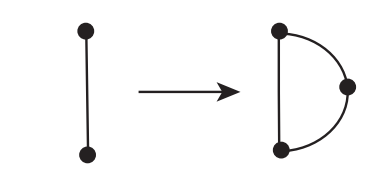
\includegraphics[width=0.2\textwidth]{A3_1.png}
\end{figure}

\begin{mdframed}
        % 4 b )
        \textit{Solution.}\\
        To prove this question is in NP-complete, two facts have to shown: it is (in)
        \begin{itemize}
            \item NP
            \item NP-hard
        \end{itemize}
        Since in q4 a), the question has been shown in NP, the only statement needs to be proven is that the question is NP-hard, that is, all NP problems can be reduced to this question in polynomial time. To shown it is NP-hard, prove a NP-complete problem, \textbf{ConnectedVertexCover} is p-reducible to this question, that is, \textbf{ConnectedVertexCover} $\leq_p$ \textbf{FriendlyRepresentative}.\\
        \\
        Given a graph $G = (V = N, E = F)$ (building such a graph $G$ by such $V$ and $F$ takes about $O(|V| + |E|) = O(n^2)$ since $F \in N \cdot N$ and $|N \cdot N| \in O(n) \cdot O(n) = O(n^2)$) and $m$, to find a correct output of a coonected vertex cover instance with $G$ and $m$ above, add a dummy node to beyond each edge in $E$, and connect each dummy node to two vertices of the edge to form a new graph $G' = (V', E')$, $V' = V \cup \{all \; dummy \; nodes\}$, $E' = E \cup \{all \; new \; added \; edges\}$. Forming this new graph takes $O(n^2)$.\\
        \\
        \textbf{WTS: }There is a connected vertex cover set $|S| = m$ in $G$ iff there is a friendly representative set $|S'| = m$ in $G'$. Prove this statements in double sides.
        
        \begin{itemize}
            \item If there is a connected vertex cover set $|S| = m$ in $G$ then there is a friendly representative set $|S'| = m$ in $G'$.
            \begin{proof}
            Suppose such a set $S$ that $|S| = m$ is found in the connected vertex cover input $G$, since each edge has at least one end in $S$, then each node in $S^c = N - S$ is connected to one node in $S$. In the new graph $G'$, the input of the representative question, except for all nodes in $G$, every new added dummy nodes is also connected to one vertex in $S$ by the algorithm of building $G'$ described above, define $S = S'$, therefore each node in $S'^c$ connects to some vertex in $S'$ as wanted.
            \end{proof}
            \item If there is a friendly representative set $|S'| = m$ in $G'$ then there is a connected vertex cover set $|S| = m$ in $G$.
            \begin{proof}
            Suppose such a set $S'$ that $|S'| = m$ is found in the friendly representative input $G'$. $G'$ derives from the $G$, the input of the connected vertex cover question. $|S| = |S'| = m$ as well ($S$ is the output of the connected vertex cover question). Let $t_i$ represent the triangle formed by an edge $e_i \in G$  with the dummy node $d_i$ added to $e_i$. There are two cases to transfer $S'$ to $S$:
            \begin{itemize}
                \item None of nodes in $t_i$ in $S'$ is the dummy node, do nothing.
                \item At least one node in $t_i$ are in $S'$ and one node is the dummy node, remove the dummy node and add a node in $G$ but not in $s'$ to $S'$.
                \item The $t_i$ only has its dummy node in $S'$, remove the dummy node and add one node the dummy connects to into $S'$.
            \end{itemize}
            All triangles has one edge that does not have the dummy node as its end points, we call this edge $e_i$ for $t_i$.Since all nodes in $S'^c$ are connected to at least one vertex in $S'$, then we can say each vertex in $S'$ contributes one or no $e_i$ in its triangle $t_i$ (contributing no $e_i$ iff the node is the dummy node and there is no in the same $t_i$ with this dummy node). Therefore, with this transformation, we should make every  $e_i$ connect to at least one node in $S$ by transferring $S'$ to $S$.\\
            It is impossible that none of nodes in $t_i$ is not in $S'$, because the dummy node in $t_i$ connects to no nodes outside of $t_i$. If the dummy node is in $S'^c$, then it connects to no nodes in $S'$, which fails the requirement of the friendly representative question. And also, this transformation leaves $|S| = m$ since once a node is removed, a new node is added or no removal happens. Also, the added new node is in $G$, thus all vertices in $S$ are in $G$.\\
           For the first case, it guarantees it contributes the $e_i$ in $t_i$ connects to a vertex in $S$ since all nodes in $t_i$ is not the dummy node, which means they must be in $G$.\\
           For the second case, since the dummy node is not in $G$, the dummy node should not appear in $S$, thus we need to remove it. Also, the number of vertices in $S$ should not change (i.e., $|S| = |S'| = m$), thus we add a new vertex in $G$ to $S$, this is proper because the all vertices in $S$ should be in G.\\
           For the third case, the transformation makes $e_i$ connected by at least one vertex in $S$ since the new added vertex to $S'$ is in G. Also, in the third case, since no node in $t_i$ makes $e_i$ has one node in $G$, thus a node connects to the dummy node should be added since this new added node is in $G$ (all nodes connected by the dummy node is in $G$).\\
           Therefore, after the transformation, every $e_i$ connects to at least one node in $S = S'$, and $|S| = |S'| = m$ as wanted.
            \end{proof}
        \end{itemize}
        By both sides of the implication, we derive the conclusion, that is, There is a connected vertex cover set $|S| = m$ in $G$ iff there is a friendly representative set $|S'| = m$ in $G'$.\\
        Also, by the discussion about forming a new graph, transferring a connected vertex cover problem to a friendly representative problem takes polynomial worst-case time $O(n^2)$, and the algorithm of friendly representative problem can be used to solve the connected vertex cover problem with the transformation. Therefore, \textbf{ConnectedVertexCover} $\leq_p$ \textbf{FriendlyRepresentative}, which means \textbf{FriendlyRepresentative} is a NP-hard problem as well. Since \textbf{FriendlyRepresentative} is both in NP and is NP-hard, then \textbf{FriendlyRepresentative} is NP-complete as wanted.
    \end{mdframed}
\end{document}